\documentclass[12pt,a4paper]{article}
\usepackage[T1]{fontenc}
\usepackage{palatino}

\usepackage{amsmath}
\usepackage{graphicx}
\usepackage{hyperref}
\graphicspath{{images/}}
\usepackage[italian]{babel}
\title{Sistema di detection di rifiuti plastici su specchi d'acqua}
\author{De Ramundo Marco - Perani Xavier}
\date{Agosto 2024}


\begin{document}
\maketitle
\section*{Abstract}
Obiettivo: ottenere un modello che possa individuare e classificare oggetti sulla superficie di uno specchio d'acqua come un fiume 
o un lago per poter riconoscere e individuare rifiuti plastici come bottiglie e buste di plastica.

\section*{Introduzione}

L'inquinamento ambientale dovuto ai rifiuti plastici è un problema che influisce tutti noi, nella fattispecie per quanto riguarda la salvaguardia 
degli oceani. Le due principali fonti di inquinamento di plastica negli oceani deriva dalla pesca e dai rifiuti gettati nei fiumi. 
Per poter contrastare la seconda causa è necessario poter effettuare operazioni di monitoraggio per prevenire che rifiuti dannosi 
possano raggiungere il mare mentre per la prima occorrono strumenti che rendano il recupero dei rifiuti più semplice e meno dispendioso. 
Anche solo riconoscere, identificare e individuare i rifiuti darebbe una grossa mano allo scopo. Per questo motivo può aver senso adoperare soluzioni 
quali modelli convoluzionali per effettuare detection degli oggetti in questione per poi agire di conseguenza con la raccolta e 
la rimozione dall'acqua della plastica.
\section*{Dataset e modello}

Il dataset scelto per il nostro scopo è \href{https://huggingface.co/datasets/kili-technology/plastic_in_river}{kili-technology/plastic\_in\_river}
che raccoglie immagini di laghetti e bacini d'acqua con oggetti e/o rifiuti sulla superficie. 
Il dataset è stato creato per la \href{https://kili-technology.com/data-labeling/machine-learning/kili-s-community-challenge-plastic-in-river-dataset}{Kili's Community Challenge},
sfida nata per invogliare la community di sviluppatori a sfruttare i modelli di deep learning per contrastare il problema dell'inquinamento degli oceani. 
La sfida si è svolta nel febbraio 2022 e il dataset è rimasto accessibile pubblicamente dopo la fine 
dell'evento\footnote[1]{Attualmente (luglio-agosto 2024) si riscontrano \href{https://huggingface.co/datasets/kili-technology/plastic_in_river/discussions/2}{problemi} nell'acquisizione del dataset tramite API. Probabilmente il proprietario del dataset 
ha spostato o tolto il dataset dal proprio server. Per il momento non si sa se il dataset tornerà a disposizione senza problemi}. 

Il dataset è composto da un totale di 4259 immagini, già divisi in tre sottoinsiemi per training, validazione e test. Nella tabella di seguito 
è possibile vedere la ripartizione delle istanze per sottoinsieme. Ogni immagine ha anche un file di testo con 
la lista degli oggetti presenti all'interno, classe dell'oggetto e posizione spaziale rispettando il data format usato da YOLO.

\begin{center}
    \begin{tabular}{ |c||c| } 
     \hline
     \textbf{Subset} & \textbf{Numero istanze} \\ 
     \hline
     Train & 3407 \\ 
     Val & 425 \\ 
     Test & 427 \\ 
     \hline
     Totale & 4259 \\
     \hline
    \end{tabular}
    \end{center}

Le categorie a disposizione per poter classificare gli oggetti identificati sono 4 e sono:

\begin{itemize}
    \item \verb+PLASTIC_BAG+
    \item \verb+PLASTIC_BOTTLE+
    \item \verb+OTHER_PLASTIC_WASTE+
    \item \verb+NOT_PLASTIC_WASTE+
\end{itemize}

La distribuzione delle classi tra le istanze non è uniforme ed è uno dei possibili problemi da affrontare durante l'addestramento del modello.
Il rischio è quello di avere difficoltà nel riconoscimento delle categorie che sono meno rappresentate all'interno del dataset.
Nella seguente tabella è possibile vedere il numero di istanze per classe all'interno dei vari subsets.

\begin{center}
    \begin{tabular}{ |c|c|c|c| } 
    \hline
    \textbf{Classe} & \textbf{Train} & \textbf{Val} & \textbf{Test} \\ 
    \hline
    \verb+PLASTIC_BAG+ & 1250 & 167 & 85 \\ 
    \verb+PLASTIC_BOTTLE+ & 6276 & 785 & 854 \\ 
    \verb+OTHER_PLASTIC_WASTE+ & 3345 & 296 & 122 \\ 
    \verb+NOT_PLASTIC_WASTE+ & 1414 & 212 & 111 \\
    \hline
    \end{tabular}
\end{center}

\newpage
\section{Modello per Object Detection}

L'obiettivo del lavoro è quello di effettuare detection sui rifiuti plastici
su immagini e per questo si è optato su una architettura basata su rete convoluzionale che allo stato dell'arte sia efficacie e abbia anche 
facilità nell'utilizzo. La scelta è ricaduta su YOLO, You Only Look Once, in
quanto risulta una delle architetture più utilizzate ed performanti.
A maggior ragione, il dataset a nostra disposizione era già predisposto per 
essere compatibile con YOLO.

Ci siamo basati sulla libreria YOLO di \href{https://docs.ultralytics.com/}{ultralytics} in quanto possiede molti metodi e strumenti per lavorare al meglio con il modello. In particolare molto utile la gestione interna per 
fare augmentation direttamente durante la fase di training.

All'inizio del progetto era a disposizione la versione 8 di YOLO che è stata
poi la versione da noi utilizzata sebbene in questi ultimi mesi sono state 
presentate le versioni 9 e 10. Abbiamo preferito mantenere per continuità con il lavoro la versione 8, che di recente ha visto anche l'aggiornamento
alla versione 8.2, una versione che mantiene la stessa struttura per quanto
riguarda l'architettura ma ha performance migliori.



\subsection*{Architettura di YOLOv8}

L'architettura di YOLOv8 si basa su un approccio end-to-end che suddivide l'immagine in una griglia e applica convoluzioni multiple per predire le bounding box e le classi degli oggetti all'interno di ciascuna cella della griglia. YOLOv8 utilizza tecniche avanzate come la \textit{Path Aggregation Network} (PANet) per migliorare l'integrazione delle informazioni a diversi livelli di profondità della rete, il che è fondamentale per rilevare oggetti di varie dimensioni e scale. Nella figura \ref*{fig:2} è riportato un diagramma semplificato dell'architettura.

\begin{figure}[h!]
    \centering
    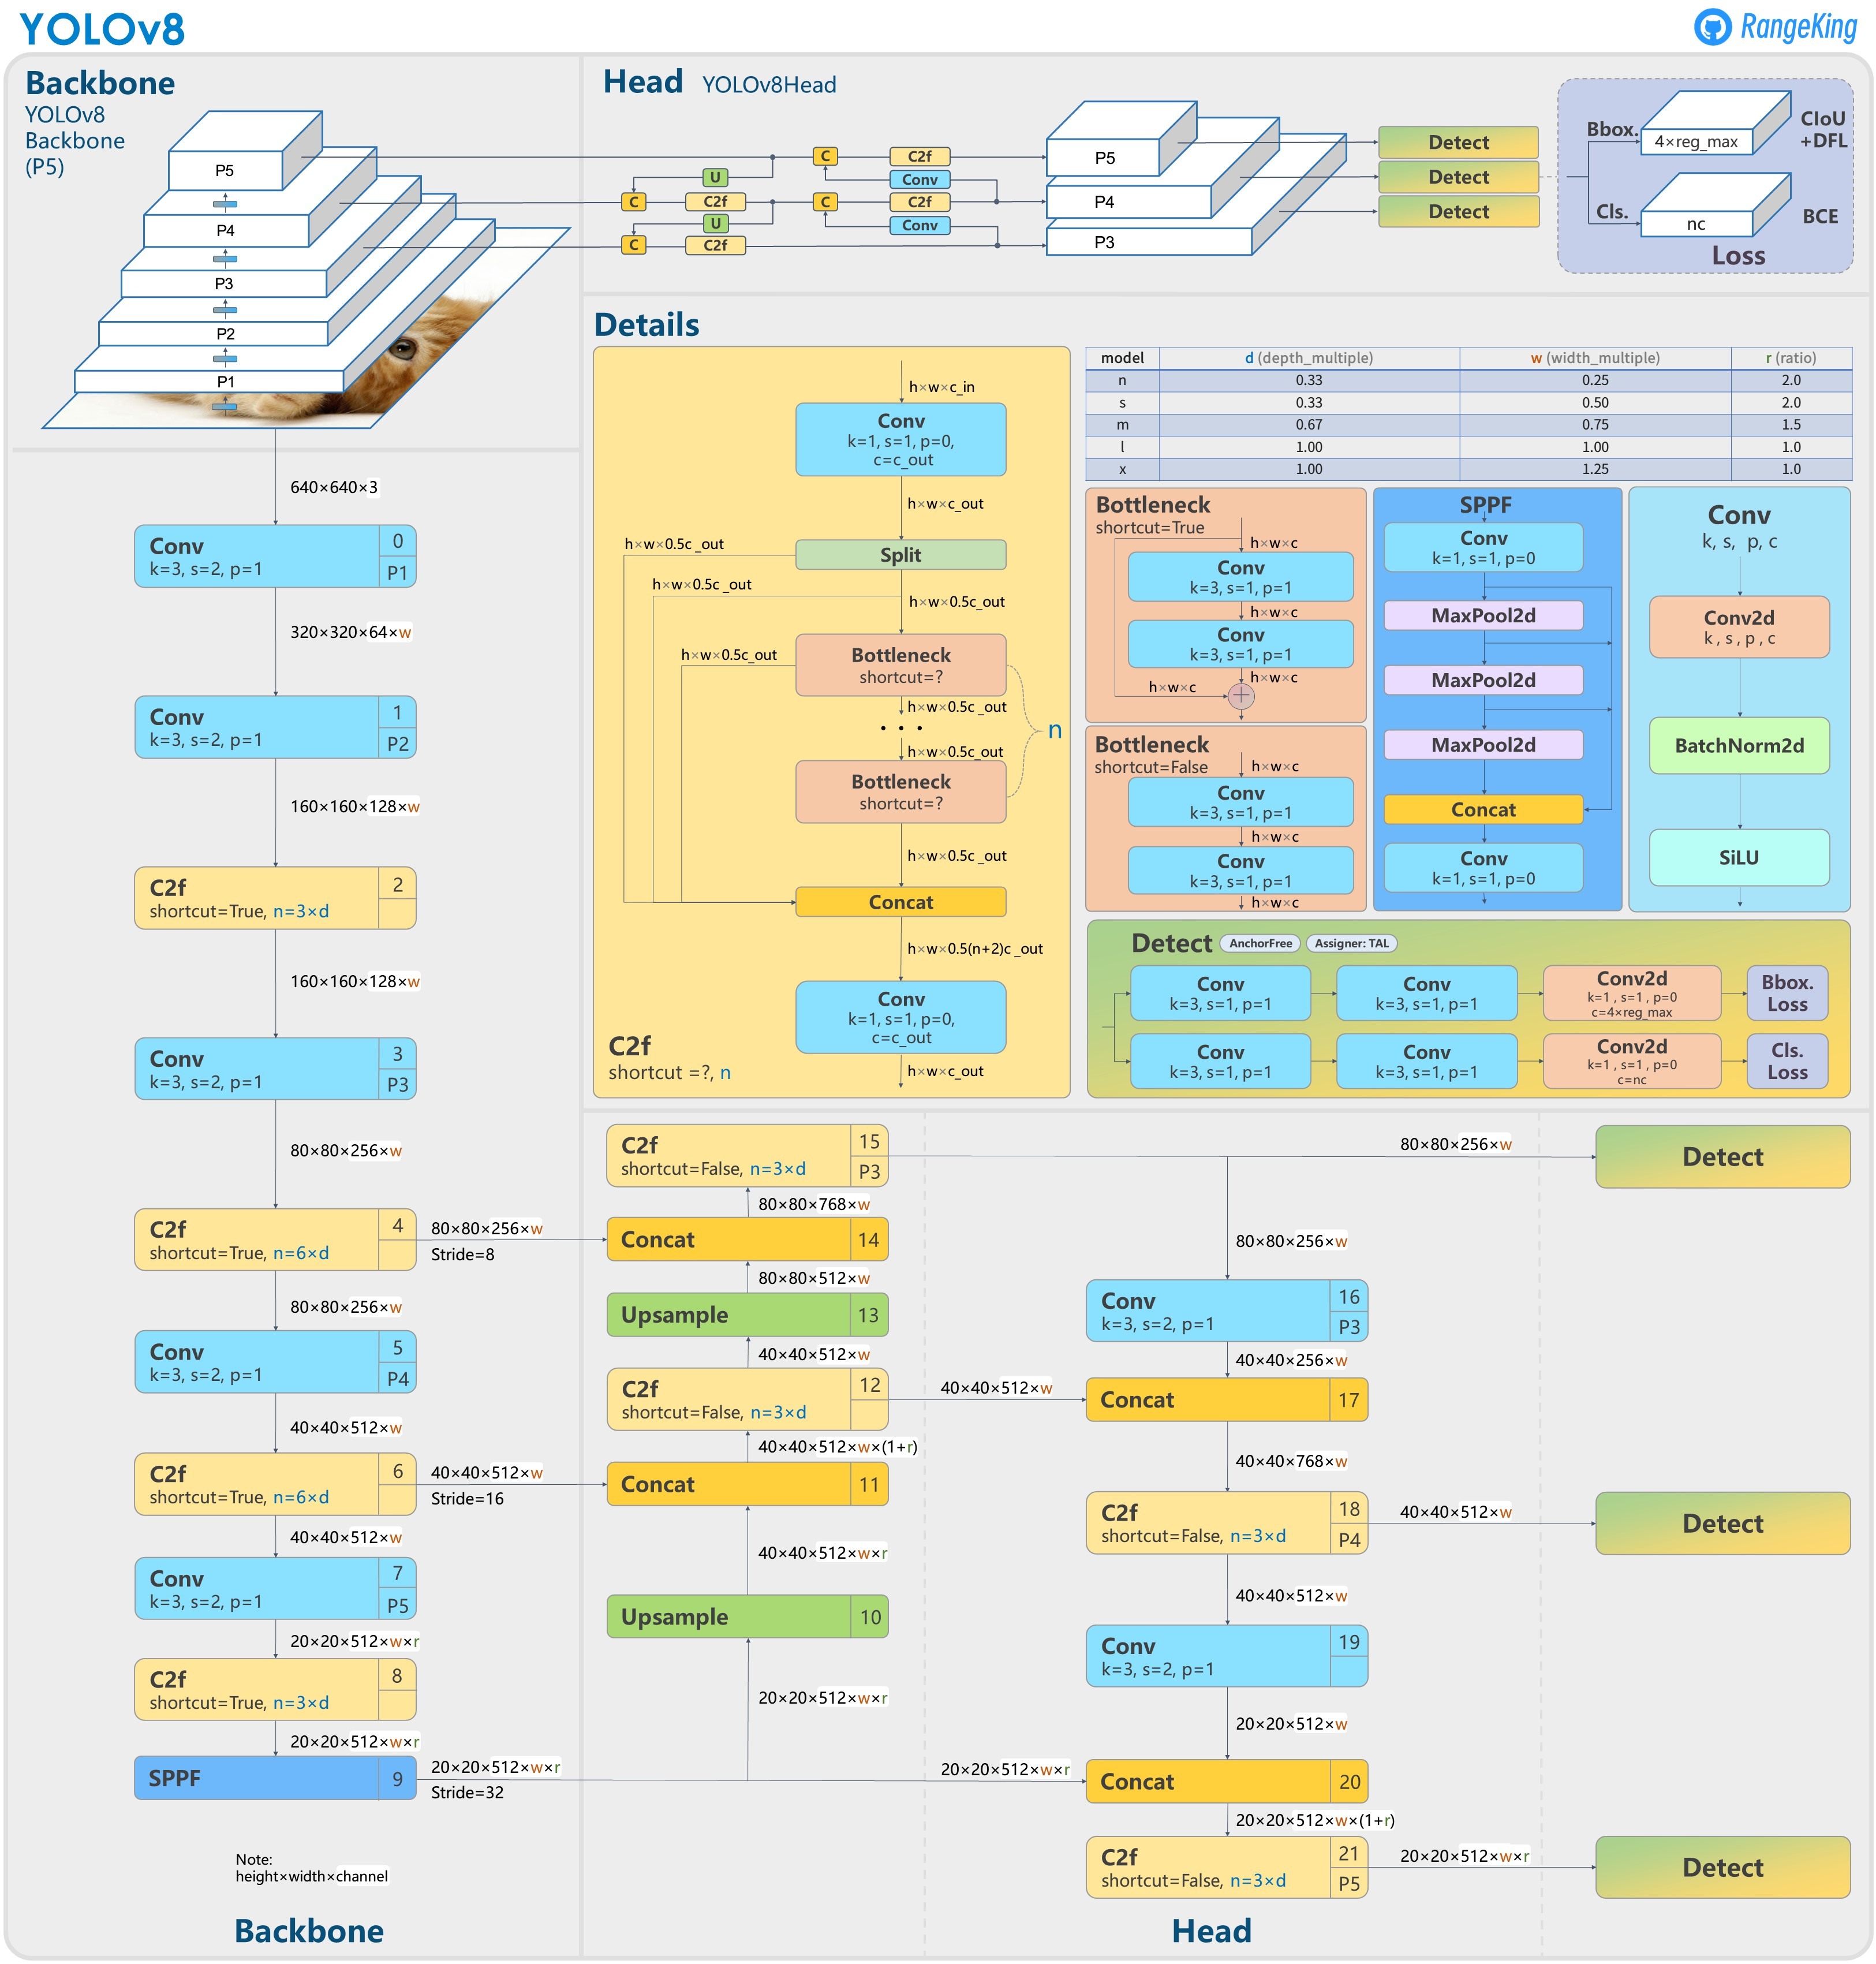
\includegraphics[width=\textwidth]{yolov8_architecture.jpg}
    \caption{Schema dell'architettura di YOLOv8}
    \label{fig:2}
\end{figure}

Il modello YOLOv8 incorpora anche una \textit{Neck} e una \textit{Head} ottimizzati per massimizzare la capacità di rilevamento attraverso una migliore aggregazione delle caratteristiche e una maggiore flessibilità nelle predizioni finali. L'uso di meccanismi come le \textit{Depthwise Separable Convolutions} contribuisce a ridurre il numero di operazioni computazionali, mantenendo un'elevata capacità espressiva del modello.

\subsection*{Dimensioni delle architetture usate}

Nell'ambito del progetto, si è scelto di utilizzare le varianti \textbf{small}, \textbf{medium} e \textbf{nano} di YOLOv8 per il task di object detection, in quanto queste architetture offrono un buon compromesso tra capacità computazionale e performance, risultando particolarmente adatte per l'esecuzione su hardware con risorse limitate quali quelle a noi disponibili.

\subsection*{Vantaggi di YOLOv8 per il Riconoscimento dei Rifiuti Plastici}

La scelta di YOLOv8 per il riconoscimento dei rifiuti plastici nei fiumi è giustificata da diversi fattori:

\begin{itemize}
    \item \textbf{Rilevamento in Tempo Reale}: YOLOv8 è noto per la sua capacità di eseguire object detection in tempo reale, il che è cruciale per applicazioni di monitoraggio continuo nei fiumi. La possibilità di rilevare e classificare i rifiuti plastici in tempo reale consente interventi immediati, riducendo il rischio che i rifiuti possano propagarsi ulteriormente.
    
    \item \textbf{Efficienza Computazionale}: Le versioni di YOLO sono ottimizzate per girare su hardware con risorse limitate, come droni o sistemi embedded. Questo le rende particolarmente adatte per applicazioni sul campo, dove la potenza di calcolo potrebbe essere un vincolo.
    
    \item \textbf{Accuratezza Elevata}: Nonostante la sua velocità, YOLOv8 mantiene un'accuratezza competitiva grazie all'uso di tecniche avanzate come l'addestramento con \textit{label smoothing} e l'adozione di una griglia più fine per la previsione delle bounding box. Questo è essenziale per distinguere efficacemente i rifiuti plastici da altri detriti naturali presenti nei fiumi, come è possibile vedere in un esempio alla figura \ref*{fig:3}.
\end{itemize}

\begin{figure}[h!]
    \centering
    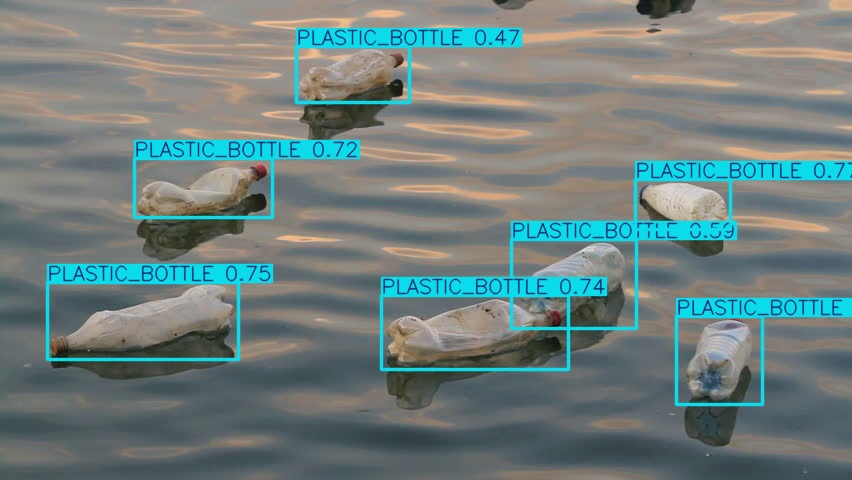
\includegraphics[width=\textwidth]{res_1203_1.jpg} 
    \caption{Esempio di output di YOLOv8 per il rilevamento di rifiuti plastici nei fiumi.}
    \label{fig:3}
\end{figure}

\newpage
\section{Metriche per valutazione performance}

Nell'ambito del riconoscimento automatico dei rifiuti plastici nei fiumi utilizzando la rete convoluzionale YOLO (You Only Look Once), l'accurata valutazione delle performance del modello è cruciale. Il contesto operativo, caratterizzato da variabilità ambientali e la presenza di oggetti confondenti, rende fondamentale l'impiego di metriche di valutazione che forniscano una visione completa dell'efficacia del modello. In questa sezione, discuteremo in dettaglio le metriche principali utilizzate per valutare il modello, giustificando la loro rilevanza rispetto all'obiettivo specifico di riconoscimento dei rifiuti plastici.

\subsection*{Precision}

La \textit{Precision} è una metrica fondamentale nel contesto del riconoscimento dei rifiuti plastici. Questa misura indica la percentuale di rifiuti classificati correttamente tra tutti quelli identificati come rifiuti dal modello. In altre parole, la precision ci dice quanto possiamo fidarci delle predizioni positive effettuate da YOLO. La formula per calcolarla è la seguente:
\begin{equation}
\text{Precision} = \frac{TP}{TP + FP}
\end{equation}
dove:
\begin{itemize}
    \item \textit{TP} (True Positive): il numero di rifiuti plastici correttamente rilevati dal modello;
    \item \textit{FP} (False Positive): il numero di oggetti non plastici erroneamente identificati come rifiuti plastici.
\end{itemize}

Nel contesto dei fiumi, dove possono essere presenti detriti naturali o altre forme di inquinamento, una precision elevata è essenziale per ridurre i falsi allarmi. Un'elevata precision significa che il modello è in grado di distinguere efficacemente i rifiuti plastici da altri oggetti, riducendo il rischio di identificare erroneamente materiali innocui come inquinanti, il che è cruciale per evitare sprechi di risorse in operazioni di pulizia.

\subsection*{Recall}

La \textit{Recall} misura la capacità del modello di identificare correttamente tutti i rifiuti plastici presenti. La recall è particolarmente importante in scenari dove la priorità è minimizzare il numero di rifiuti plastici non rilevati (falsi negativi), che possono avere un impatto ambientale significativo se lasciati nei corsi d'acqua. La formula per calcolare la recall è la seguente:
\begin{equation}
\text{Recall} = \frac{TP}{TP + FN}
\end{equation}

Nel contesto del riconoscimento dei rifiuti plastici, un alto valore di recall significa che il modello è efficace nel rilevare la maggior parte dei rifiuti, riducendo al minimo il rischio che rifiuti plastici possano sfuggire all'attenzione. Tuttavia, un aumento della recall potrebbe portare a una diminuzione della precision, poiché il modello potrebbe iniziare a classificare erroneamente più oggetti come plastica per evitare di perdere i rifiuti effettivi. Pertanto, è fondamentale trovare un equilibrio tra precision e recall.

\subsection*{F1-Score}

L'\textit{F1-Score} è la media armonica tra precision e recall, offrendo una misura bilanciata che tiene conto sia dei falsi positivi che dei falsi negativi. Questa metrica è particolarmente utile in scenari come il riconoscimento dei rifiuti plastici, dove il dataset può presentare classi sbilanciate e dove è importante non sovra-ottimizzare il modello per una sola metrica a scapito dell'altra. La formula per l'F1-Score è:
\begin{equation}
F1 = \frac{2 \cdot \text{Precision} \cdot \text{Recall}}{\text{Precision} + \text{Recall}}
\end{equation}

Nel contesto del riconoscimento dei rifiuti plastici, l'F1-Score è \textbf{particolarmente indicato}, poiché consente di valutare l'efficacia complessiva del modello, bilanciando l'accuratezza con la capacità di rilevamento. Un F1-Score elevato indica che il modello YOLO è in grado di mantenere un buon equilibrio tra identificare correttamente i rifiuti plastici e minimizzare gli errori.

\subsection*{mean Average Precision (mAP)}

Il \textit{mean Average Precision} (mAP) è una delle metriche più utilizzate e riconosciute nella valutazione delle performance di modelli di \textit{object detection}. Il mAP rappresenta la media delle \textit{Average Precision} (AP) calcolate su tutte le classi considerate nel modello. La \textit{Average Precision}, a sua volta, è l'area sotto la curva Precision-Recall per ciascuna classe. Il mAP è particolarmente rilevante per il nostro caso di studio, poiché:

\begin{itemize}
    \item Riflette le prestazioni complessive del modello su più classi di rifiuti plastici (se categorizzati in diverse tipologie);
    \item Tiene conto della capacità del modello di rilevare i rifiuti plastici in condizioni variabili, come differenti condizioni di illuminazione, presenza di acqua torbida, e variazioni nella forma e dimensione dei rifiuti;
    \item Considera le variazioni nella soglia di rilevamento del modello, fornendo un'indicazione della sua robustezza e capacità di generalizzazione.
\end{itemize}

Nel caso del riconoscimento dei rifiuti plastici, un mAP elevato indica che il modello è in grado di rilevare correttamente i rifiuti in diverse situazioni operative, mantenendo un buon equilibrio tra precisione e richiamo per ciascuna classe considerata. Questo è cruciale per garantire che il sistema di monitoraggio automatico sia affidabile in ambienti reali e possa contribuire efficacemente alla riduzione dell'inquinamento nei corsi d'acqua.

\end{document}